
%% LLT: Turn off some annoying warnings...
\RequirePackage{silence}
\WarningFilter{titlesec}{Non standard sectioning command}
\WarningFilter{scrreprt}{Usage of package}
\WarningFilter{scrreprt}{Activating an ugly workaround}

% *********************************************************
% CHOOSE THEME (ucph, sund, science, hum, samf, jura, teo)
% *********************************************************
\newcommand{\thesisTheme}{ucph} % to colortheme and titlepage image
\newcommand{\frontpageimage}{cover_image.png} % cover image

\DeclareUnicodeCharacter{0308}{HERE!HERE!} % I had issues with this character ...
% *********************************************************
% DOCUMENT CLASS
% *********************************************************
\documentclass[%
	paper=B5,					% paper size
	11pt,						% font size
	twoside=true,				% two-sided printing
	openright,					% doublepage cleaning ends up right side
	parskip=full,				% spacing value / method for paragraphs, half*, half, half-
	chapterprefix=true,			% prefix for chapter marks
	headings=normal,			% size of headings
	bibliography=totoc,			% include bib in toc
	listof=totoc,				% include listof entries in toc
	titlepage=on,				% own page for each title page
	captions=tableabove,		% display table captions above the float env
	draft=false,				% value for draft version
	abstract=on,                % abstract title on/off
]{scrreprt}
\usepackage[utf8]{inputenc}
\usepackage[english]{babel}     % adjust the language

% **************************************************
% COMMANDS FOR REUSE
% **************************************************

% Thesis
\newcommand{\thesisTitle}{YOUR TITLE}
\newcommand{\thesisSubtitle}{YOUR SUBTITILE}
\newcommand{\thesisName}{NAME SURNAME}
\newcommand{\thesisSubject}{PhD thesis}
\newcommand{\thesisDate}{\today}
\newcommand{\thesisVersion}{v240208}

% Supervisors & Collaborators

\newcommand{\thesisPrincipalSupervisor}{SUPERVISOR}
\newcommand{\thesisCoSupervisor}{COSUPERVISOR}
\newcommand{\thesisExternalSupervisor}{External Supervisor}
\newcommand{\thesisMainInstitut}{Novo Nordisk Foundation Center for Metabolic Research, University of Copenhagen}
% \newcommand{\thesisCollab}{If any?}

% University of Copenhagen
\newcommand{\thesisUniversity}{\protect{University of Copenhagen}}
\newcommand{\thesisFaculty}{Faculty of Health and Medical Sciences}
\newcommand{\thesisInstitute}{PhD}
\newcommand{\thesisCity}{Copenhagen N}
\newcommand{\thesisAddress}{Blegdamsvej 3B}
\newcommand{\thesisPostal}{2200}

% **************************************************
% MY COMMANDS and packages
% **************************************************
\newcommand{\doi}[1]{\href{https://doi.org/#1}{#1}}     % Have dois as links
\newcommand{\https}[1]{\href{https://#1}{#1}}            % make any https link
%\usepackage{enumitem}                                   % Make item lists without numbers/bullets - already included in ucphthesis, therefore commented out here
\usepackage{dirtytalk}                                  % In-line quotations using \say{}
\usepackage{multirow}                                   % Multirow in table
\usepackage{graphicx}                                   % More table stuff
\usepackage{makecell}                                   % Get linebreak in table cell
\usepackage{tcolorbox}                                  % Make a colored box
\definecolor{colorforbox}{RGB}{247,249,254}             % color for colored box
%\renewcommand*{\bibfont}{\normalfont\footnotesize}       % change size of bibliography. footnotesize can be used for a bit smaller size.
\usepackage{amsmath}                                    % for making equations
\usepackage[symbol]{footmisc}                           % make symbols available for footnote
\renewcommand{\thefootnote}{\fnsymbol{footnote}}        % change footnote to use symbols. Symbol numbers found here: https://tex.stackexchange.com/questions/826/symbols-instead-of-numbers-as-footnote-markers
\usepackage{wrapfig}                                    % Have text wrap around figures (used for QR code in BALDR intro)

\usepackage{pdfpages}                                   % Insert pdfs
	\includepdfset{
		pages = {1-}, % from page 1 to the final page
		pagecommand = {}, % uses global document layout
		frame = true, % draw discrete border around page
		offset = 0mm 0mm, % outward/upward
		scale = 0.84,
    link=true, % allow pointing to inserted pages
    rotateoversize % rotates landscape pages
	}
 \newcommand{\includepdfsupp}{                         % Insert supplementary pdf
  \includepdf[
    nup=1x2, 
    delta=0mm 2mm, 
    angle=-90, 
  ]
    }

\newtcolorbox[auto counter,number within=chapter]{bluebox}[2][]{ % Make blue boxes.
toptitle=3mm, colback=colorforbox, colframe=colorforbox, coltitle=black, 
titlerule=1mm, fonttitle=\bfseries\sffamily, fontupper=\sffamily\small, 
sharp corners, float, floatplacement=t,
title=Box~\thetcbcounter~#2, #1}

\newcommand\blankpagenumbered{%
    \null
    \thispagestyle{plain}%
    \addtocounter{page}{-1}%
    \newpage}

% *********************************************************
% PACKAGES
% *********************************************************
\usepackage[					% UCPH thesis style
    figuresep=colon,        
    sansserif=false,        
    hangfigurecaption=false,
    hangsection=true,       
    hangsubsection=true,
    hangsubsubsection=true,
    colorize=full,          
    colortheme={\thesisTheme},  % ucph, sund, science, hum, etc.?
    bibsys=biber,
    bibfile=references,       % defines your .bib file
    bibstyle=authoryear,      % refer to https://da.overleaf.com/learn/latex/Biblatex_citation_styles
]{ucphthesis}
\hypersetup{					% setup the hyperref-package options
	pdftitle={\thesisTitle},	% 	- title (PDF meta)
	pdfsubject={\thesisSubject},% 	- subject (PDF meta)
	pdfauthor={\thesisName},	% 	- author (PDF meta)
	plainpages=false,			% 	-
	colorlinks=true,			% 	- colorize links
        citecolor=[RGB]{188 60 48},
        linkcolor=[RGB]{188 60 48},
        anchorcolor=.,
        filecolor=.,
        menucolor=.,
        runcolor=.,
        urlcolor=[RGB]{188 60 48},
        pdfborder={0 0 0},			% 	-
	breaklinks=true,			% 	- allow line break inside links
	bookmarksnumbered=true,		%
	bookmarksopen=true			%
    }

% *********************************************************
% Cover page content
% *********************************************************
%\subject{\vspace{4.5cm} \thesisSubject}
\title{\thesisTitle}
\author{\thesisName}
\date{\thesisDate}


% ********************************************************* 
% THESIS CONTENT
% *********************************************************
\begin{document}

\begingroup
  \fontencoding{T1}\fontfamily{LinuxLibertineT-OsF}\selectfont
  \makekutitle
\endgroup

% -------------------------- 
% Front matter
% --------------------------
\pagenumbering{roman}
%\pagestyle{empty}				            % no header or footers
%\AddToShipoutPicture*{\TitleBackground}     % adding background picture
%\input{frontbackmatter/coverpage}
% Cover back page
\AddToShipoutPicture*{\TitleWatermark}% adding watermark
% \afterpage{\blankpage}
\title{\thesisTitle}
\date{\thesisDate}
\maketitle
\begin{fullwidth}

  \newcommand{\affiliation}[1]{{\small #1}}
  
  \thispagestyle{empty}
  \setlength{\parindent}{0pt}
  \setlength{\parskip}{\baselineskip}
  
  %
  {\Large \textbf{Author}}
  
  \textbf{\thesisName} \\
  \affiliation{Novo Nordisk Foundation Center for Protein Research, University of Copenhagen}

  %
  {\Large \textbf{Supervisors}}
  
  \textbf{\thesisPrincipalSupervisor}, Professor, PhD \\
  \affiliation{\thesisMainInstitut}\\
  \affiliation{Novo Nordisk Foundation Center for Metabolomics Research, University of Copenhagen} \\
  \affiliation{The Novo Nordisk Foundation Center for Genomic Mechanisms of Disease, Broad Institute of MIT and Harvard} \\
  (Principal Supervisor)\vspace{0.4em}\\
  \textbf{\thesisCoSupervisor}, Professor, PhD \\
  \affiliation{\thesisMainInstitut} \\
  (Primary Co-supervisor) \vspace{0.4em} \\
  \textbf{\thesisExternalSupervisor}, Professor, PhD \\
  \affiliation{Novo Nordisk Foundation Center for Metabolomics Research, University of Copenhagen}\\
  (External supervisor)

  %
  {\Large \textbf{Assessment committee}}
  
  \textbf{Firt Last}, Associate Professor, PhD (chair) \\
  \affiliation{\thesisMainInstitut}\vspace{0.4em}\\
  \textbf{First Last}, Associate Professor, PhD \\
  \affiliation{Department of Biotechnology and Biomedicine, Technical University of Denmark}\vspace{0.4em}\\
  \textbf{First Last}, Associate Professor, Dr.\\
  \affiliation{VIB-UGent Center for Medical Biotechnology, VIB, Belgium}\vspace{0.4em}\\
  %    
\end{fullwidth}

\pagestyle{plain}

%\vspace*{4cm}
\textit{"I want to say a word for the study of comparative physiology also for its own sake. You will find in the lower animals mechanisms and adaptations of exquisite beauty and the most surprising character, and I think nothing can be more fascinating than the senses and instincts of insects as revealed by the modern investigations."} \\
\newline
\rightline{August Krogh, 1929 \nocite{Krogh1929}} \\
\vspace{2cm}
\newline
\textit{"It is certain that there may be extraordinary mental activity with an extremely small absolute mass of nervous matter: thus the wonderfully diversified instincts, mental powers, and affections of ants are notorious, yet their cerebral ganglia are not so large as the quarter of a small pin's head. Under this point of view, the brain of an ant is one of the most marvelous atoms of matter in the world, perhaps more so than the brain of a man."} \\
\newline
\rightline{Charles Darwin, 1872 \nocite{Darwin1872TheSex}}
\vspace{3.8cm}


        % INCLUDE Quotes
\pdfbookmark[0]{Preface}{Preface}
\chapter*{\vspace{-5em}Preface}
\label{ch:preface}
\vspace{-8em}
This thesis has been submitted to the Graduate School of the Faculty of Health and Medical Sciences, University of Copenhagen. 

The work presented in this thesis was carried out at the Novo Nordisk Foundation Center for Protein Research during the period of 1st Sepember 20XX to 31th august 20xx under the supervision of Professor first last.

The work was funded by the Novo Nordisk Foundation (grants NNFXXX).


\begin{flushright}
	
	Copenhagen, August 20XX
	
	\vspace{1em}
	%\begin{figure}[h]
	%  \vspace{-\baselineskip}
	%  \includegraphics[width=0.5\textwidth, right]{figures/signature.png}
	%\end{figure} 
	%\vspace{2em}
	\thesisName
	
\end{flushright}       % INCLUDE Preface
\pdfbookmark[0]{Acknowledgements}{Acknowledgements}
\chapter*{Acknowledgements}
\label{chap:acknowl}
\Blindtext[2] % INCLUDE Acknowledgements
\pdfbookmark[0]{Summary}{Summary}
\chapter*{Summary}
\label{chap:summary}
\Blindtext[2]      % INCLUDE summary
\pdfbookmark[0]{Dansk resumè}{Dansk resumè}
\chapter*{Dansk resumè}
\label{chap:danish summary}
\Blindtext[2]      % INCLUDE danish summary
\pdfbookmark[0]{Publications and Manuscripts}{Publications and Manuscripts}
\chapter*{Publications and Manuscripts}
\label{chap:pubs}
\addcontentsline{toc}{chapter}{Publications and Manuscripts}

\textbf{\hyperref[paper:one]{Paper I}} \\
\fullcite{Webel2023-hi} \\
In Revision, Nature Communications

\textbf{\hyperref[paper:two]{Paper II}} \\
\fullcite{Webel2023-kc} \\
Accepted, Scientific Data

\textbf{\hyperref[paper:three]{Paper III}} \\
\fullcite{Mynster_Kronborg2023-ek}

\newpage
\section*{Further contributions to articles}

\fullcite{Niu2022-el}

\fullcite{Allesoe2023-ip}

\fullcite{Dai2021-hq}

\fullcite{Jespersen2023-hc}

\fullcite{Luo2022-nu} % INCLUDE list of publications
\pdfbookmark[0]{Abbreviations}{Abbreviations}
\chapter*{List of abbreviations}
\label{chap:abbr}
\addcontentsline{toc}{chapter}{Abbreviations}
\begin{acronym}
    \acro{ICU}{intensive care unit}
    \acro{KNN}{k-nearest neighbors}
\end{acronym}
    % INCLUDE Rationale
\pdfbookmark[0]{FiguresTables}{FiguresTables}
\chapter*{Figures and Tables}
\addcontentsline{toc}{chapter}{\listfigurename}
\listoffigures
\addcontentsline{toc}{chapter}{\listtablename}
\listoftables    % INCLUDE Rationale
\clearpage


\setcounter{tocdepth}{2}		% define depth of toc
%\tableofcontents				% display table of contents
{
  \hypersetup{linkcolor=black}
  \tableofcontents
}
\clearpage


% -------------------------- 
% Main matter
% --------------------------
\pagenumbering{arabic}			% arabic page numbering
\setcounter{page}{1}			% set page counter
\pagestyle{maincontentstyle} 	% fancy header and footer

\chapter*{Thesis content and overview}
\label{thesis-content-and-overview}

The overall topic of this thesis is ... It includes both analysis of ...
The last article looks at... . All
three studies focus on ...

\textbf{Chapter \ref{chap:background}} introduces the general background elaborating on the
type of data, phenotypes and topics relevant for the included studies.
\textbf{Chapter \ref{chap:methods}} introduces the most relevant methods and technical
aspects. \textbf{Chapter \ref{chap:objectives}} outlines the objectives, while
\textbf{chapter \ref{chap:description-projects}} provides an overview of the studies. \textbf{Chapter
\ref{chap:res}} discusses results from the studies and \textbf{chapter \ref{chap:persp}} concludes
with perspectives and future ideas.
\chapter{Background}
\label{chap:intro}
\vspace{4cm}
Locomotion is the means by which animals move around the world. However, movement comes at a price. Sensory performance is decreased as motion blur hampers visual discrimination \autocites{Kramer2001, Land1999} and extraction of relevant visual information may prove more difficult \autocite{Land1999}. This is particularly important in unpredictable environments. Furthermore, it is dependent upon muscular work and it is thus inherently energetically costly. An example is the 15-50 fold increase in oxygen consumption in flying locusts compared to rest-state \autocite{Krogh1949TheFlight}.
It is thus reasonable to believe that metrics of walking are evolutionarily optimised. That would entail animals choosing walking speeds that allows extraction of visual information, such as distance cues, whilst also being energetically efficient. \\
\vspace{1cm}



In this chapter, I will review the:
\begin{itemize}[noitemsep]
    \item Evidence for visual control of locomotion
    \item Evidence for energetic control of locomotion
    \item The use of virtual reality in animal behaviour research
\end{itemize}

\vfill
\clearpage
\section{Control of locomotion}

\subsection{Optic flow: Definition and features}

Optic flow is the movement of structured light across the retina \autocite{Raudies2013}. The practical meaning of this is that optic flow does not estimate the physical speed of things but rather the speed at which they move past the eye (in degrees/s). Optic flow can be divided roughly into two parts, rotational and translational both of which can occur around all axes. Both contain information about the speed and direction of movement. Translational optic flow from forward movement is generated around a central focal point with vectors pointing in opposite directions for the two eyes. During forward motion, the flow points away from the focal point and is said to be expansive. During backwards motion, on the other hand, it points towards the focal point and is retracting. Translational optic flow provides information regarding the translational distance of movement, and also allows for inference of depth due to the relative movement of components across the visual field, called motion parallax (e.g. when an animal moves forward, the translational optic flow generated by objects nearby will be larger than that generated by objects far away). Insects like locusts and mantids use motion parallax by translating sideways (peering) without rotating, to infer distance (e.g. \cite{Sobel1990b}). In rotational optic flow, vectors are pointing in the same direction for both eyes, providing directional information. However, it does not allow for depth perception as retinal displacements are independent of the distance to the retina. As movement is often a mixture of simultaneous translation and rotation rather than pure translation, this makes efficient extraction of distance information more difficult. In this thesis, I only discuss translational optic flow unless otherwise stated.\\ \\
Optic flow was first proposed in a biological setting by Gibson in 1958 \autocite{Gibson1958a} and has since been confirmed to be behaviourally relevant in a wealth of species, including humans \autocite{Warren1988}, rats \autocite{Kautzky2016}, zebra fish \autocite{Wang2019}, crabs \autocite{Horseman2011}, bees \autocite{Linander2015}, blowflies \autocite{Longden2009} and desert ants \autocite{Pfeffer2016}. Furthermore, it has been shown to influence a multitude of behaviours such as collision avoidance, mate following, predator avoidance, feature detection and path integration (e.g. \cite{Srinivasan1996}).

Within insects, \textcite{David1982CompensationTunnel} was the first to investigate the use of optic flow in the control of locomotion speed in a series of experiments on \textit{Drosophila}. It had previously been shown that some flying insects can maintain their flight speeds constant relative to the ground \autocite{David1979OptomotorDrosophila.}. \textcite{David1982CompensationTunnel} made flies fly inside a "barber's pole" wind tunnel, enabling him to manipulate the visual motions around the flies. He was able to make the flies adopt a stable position within the tunnel by imposing a headwind in the tunnel. Flies kept a steady ground speed in head winds ranging from 0.2-1.0m/s. He then manipulated the diameter of the tunnel, the wavelength of the revolving pattern and the pitch of the revolving lines. Thus, he could infer which aspects enabled to fly to maintain a preferred speed and concluded that it was due to the optic flow.

These findings were extended to another flying species, the honey bee, by \textcite{Srinivasan1996}. They had previously shown that honey bees use optic flow in their centering response, which enables them to keep objects on either side at equal distances \autocite{Srinivasan1991RangeHoneybees}. This response is a way of keeping them from colliding with nearby objects. They now set out to investigate if optic flow was also responsible of the control of their flight speed. By showing that bees slow down when flying through a narrowing gap with vertical lines on the walls, they showed that bees do indeed use optic flow. To control that it was not confounded by the fact that closer lines appear larger, they had bees fly through a tunnel in which the lines had a short wavelength and the other had a greater wavelength. Bees showed no change of flight speed, confirming that optic flow was indeed the metric used by the bees. The findings have since also been confirmed in bumblebees \autocite{Linander2015}.  % INCLUDE Introduction
\chapter{Methods}
\label{chap:methods}

\hspace{0pt}
\vfill
\section{Animals and Animal Preparation}
Experiments were performed using wood ants (\textit{Formica rufa L.}). Colonies were collected during summer 2018 from Ashdown Forest, Sussex, UK (N 51 4.680, E 0 1.800). They were kept in large plastic containers with Fluon coated walls at 26 degrees celsius with a 12h light: 12h darkness light cycle regime. They were fed \textit{ad libitum} with 33.3\% sucrose solution. \\
For experiments, ants were chosen based on their size and level of activity (large, active ants were preferred). Subsequently, these ants were painted and placed in small groups for 30 minutes to reduce ant-ant aggression due to the paint odour before being transferred to a small portable nest-like box with unpainted nest mates. To prepare an ant for the experiment, they were first put on ice for 5-10 min to cool them reducing movement before an insect pin (Austerlitz Insect Pin) was attached to the ants back with ultraviolet-light-sensitive glue (5 Second Fix) under a microscope (Olympus Corporation, Tokyo, JP). The pin was bent to a 135\textsuperscript{o} angle about 2/3 up the pin. The ant was then transferred to a separate box where it was kept until the first trial. After the first trial the ant was transferred to nest-like box and kept for 2-4h before the second trial. Ants were picked up with tweezers by the pin and harnessed to the trackball system (described in detail later). After finishing the experiments, animals were discarded in ethanol ($\geq$ 99.8\%, Sigma-Aldrich Ltd, Dorset, UK).
\vfill
\hspace{0pt}      % INCLUDE Methods
\chapter{Research objectives}
\label{chap:objectives}

\Blindtext[2]         % INCLUDE Hypothesis
\chapter{Description of research projects}
\label{chap:description-projects}

Locomotion is thought to be a tightly controlled behaviour, ensuring good sensory performance, especially visual, and reducing energy expenditure \autocites{Benichou2011IntermittentStrategies, Kramer2001}. Whether this is the case in the wood ant \textit{Formica rufa} remains unknown, despite many aspects of ant locomotion having been well studied \autocites{Lipp2005, Wahl2015}. The wood ant is an eusocial insect capable of using vision for navigation \autocite{Harris2007} and associative learning \autocite{Fernandes2017a}. Furthermore, other ant species have been found able to use optic flow for path integration (\textit{Cataglyphis}, \citealt{Ronacher1995, Pfeffer2016}). It could thus be speculated that vision actively controls general walking features such as speed, duration and pausing in the wood ant, \textit{Formica rufa} (like bees control speed, \cite{Schone1996, Linander2015}). We ask the following question: Does control of walking speed and pausing depend on the presence and speed of optic flow?

A promising approach for performing behavioural experiments in a laboratory setting is the use of virtual reality. Insects have recently been shown to exhibit naturalistic behaviour in closed-loop within a virtual environment \autocites{Takalo2012, Buatois2017, Seelig2010}. Such setups allow data sampling at precise temporal and spatial resolution whilst animals walk unrestricted for long periods of time. They further enable the recording of brain activity directly, either by electrophysiological recordings or calcium imaging \autocite{Seelig2010}. However, despite continued efforts from multiple laboratories it has not yet been possible to make a setup in which ants will readily behave within closed-loop. Nevertheless, we set out to develop a virtual reality paradigm for wood ants (\textit{Formica rufa}). We propose a paradigm based on a modified closed-loop version of the trackball setup by \citeauthor{Dahmen2017} (\citeyear{Dahmen2017}) combined with the virtual reality software developed by \citeauthor{Aronov2014b} (\citeyear{Aronov2014b}).

\begin{figure}[h]
    \centering
    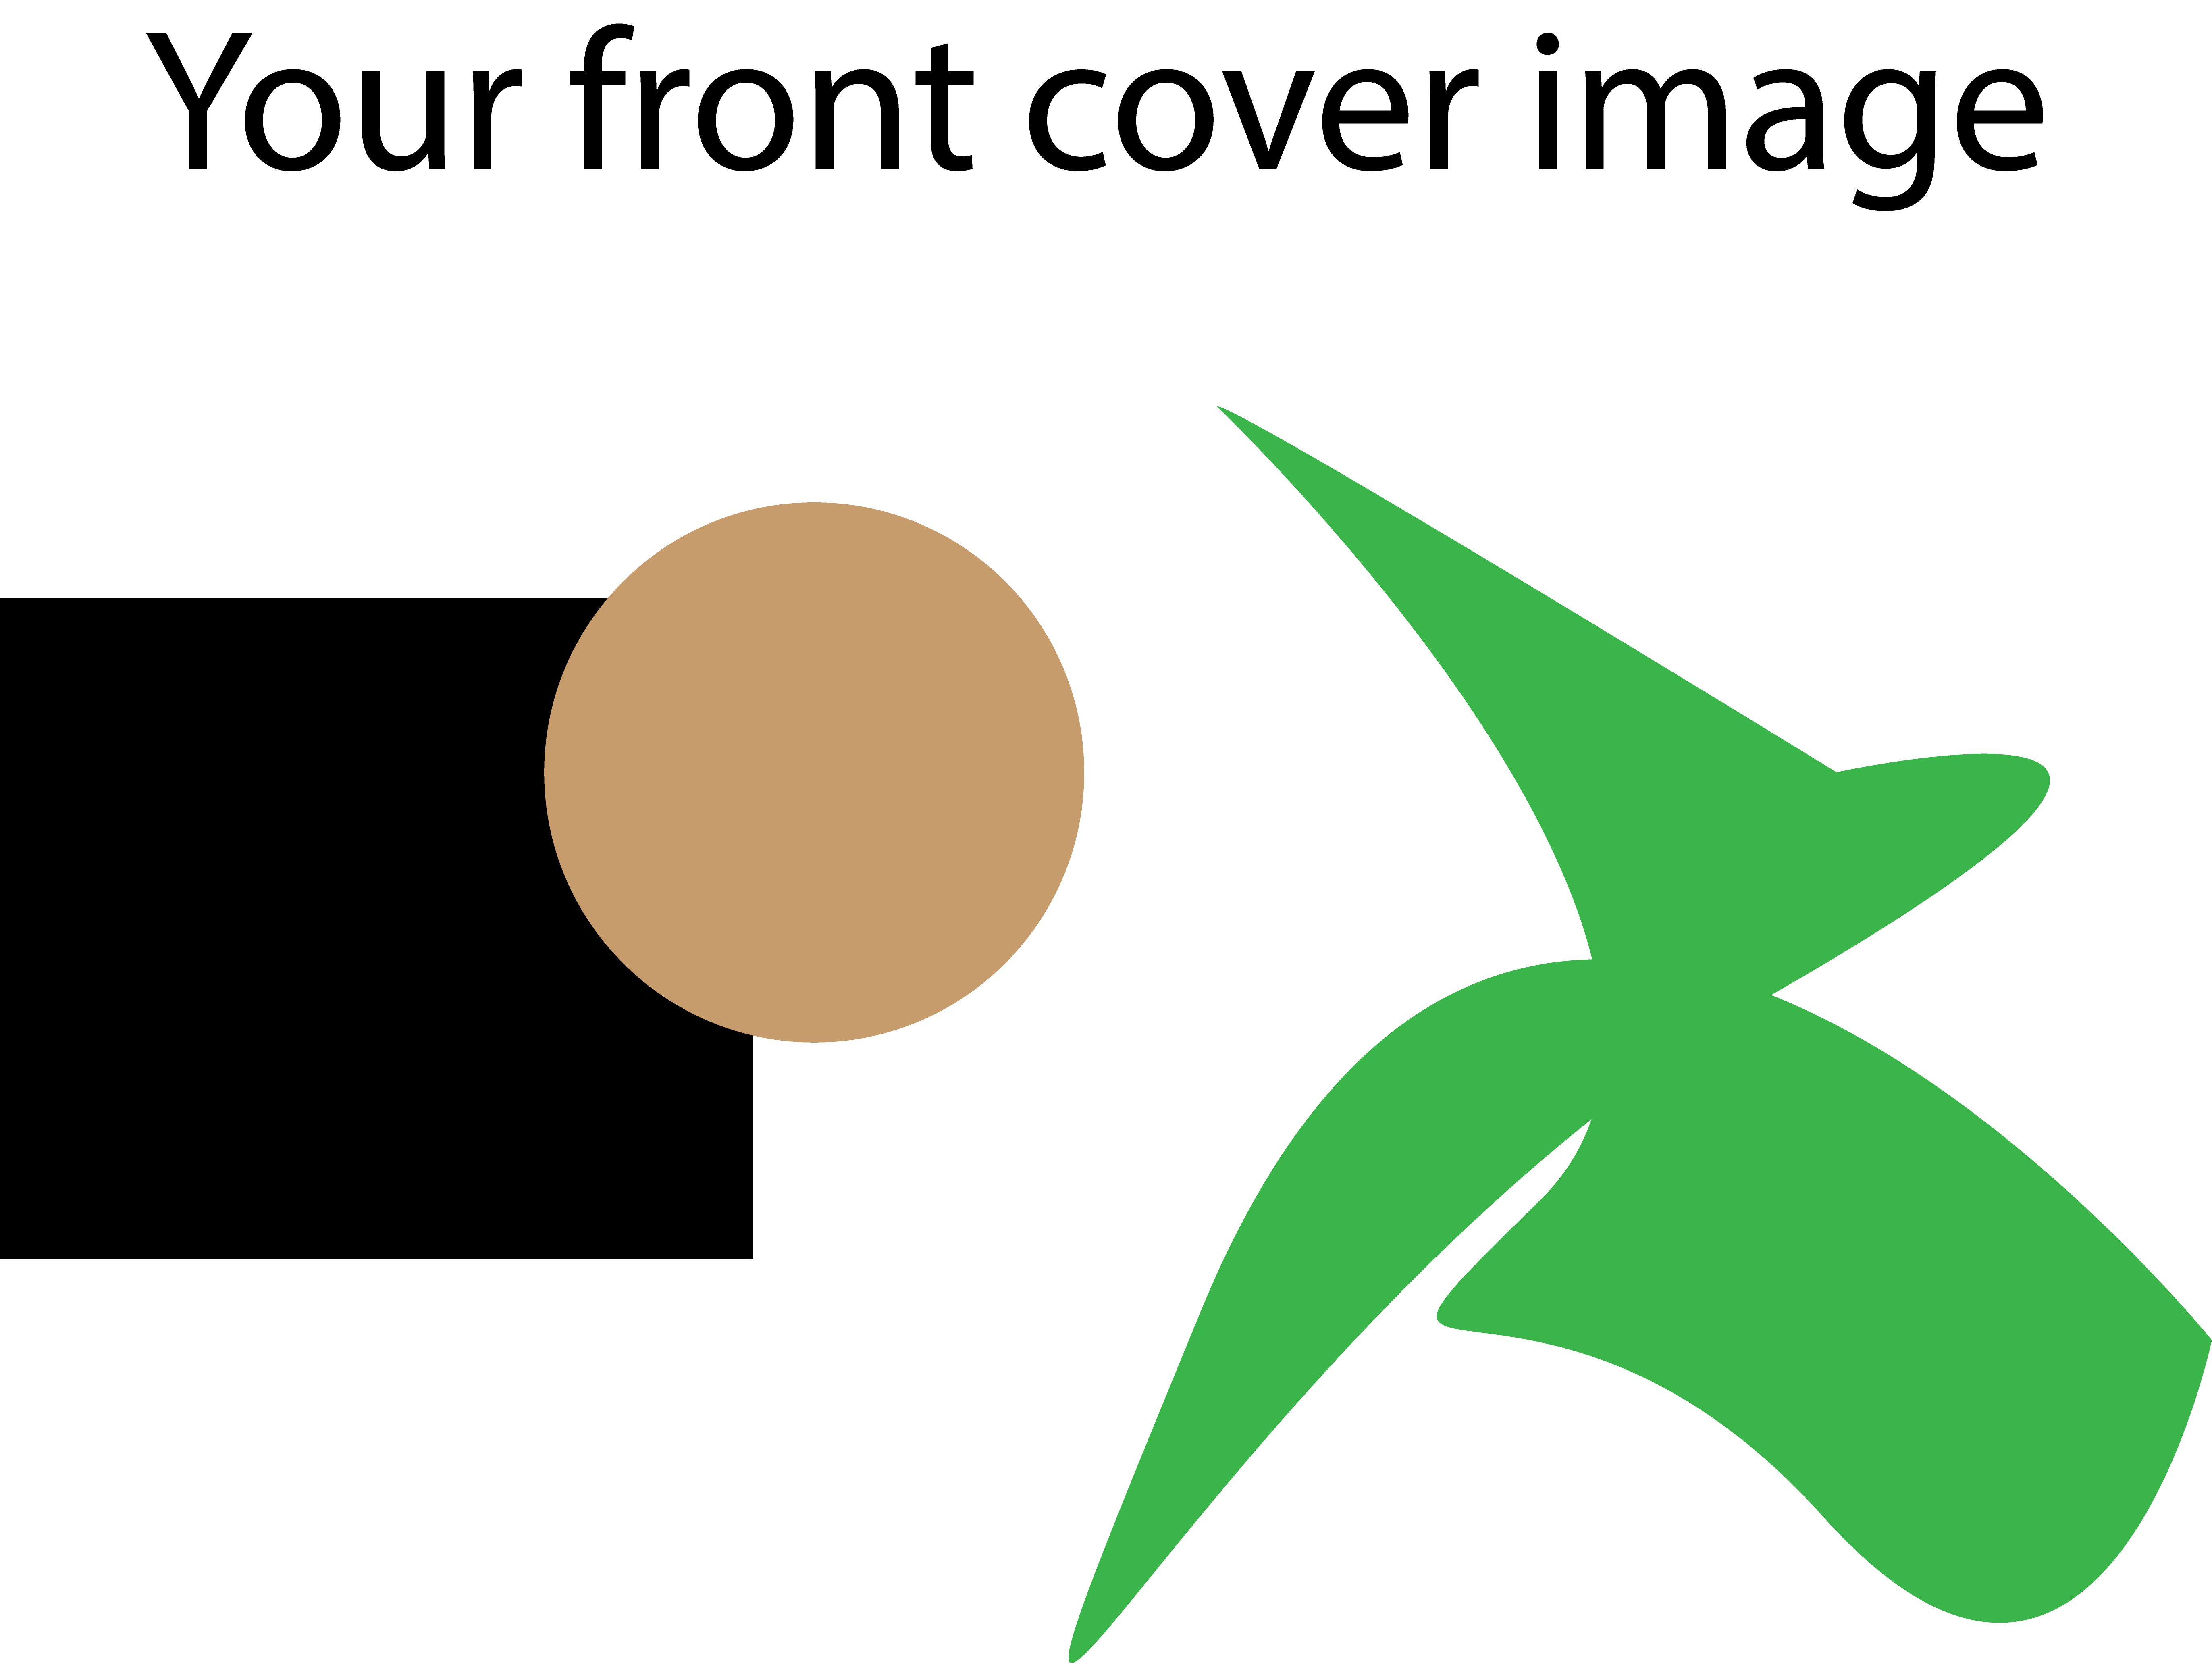
\includegraphics[width=100mm]{theme/cover_image.png}
    \caption[short image caption for list of figures]{A very long and very complicate image caption for a simple Image example.
    A very long and very complicate image caption for a simple Image example.
    A very long and very complicate image caption for a simple Image example.
    A very long and very complicate image caption for a simple Image example.
    A very long and very complicate image caption for a simple Image example.
    A very long and very complicate image caption for a simple Image example.}
    \label{fig:image_example}
\end{figure}

And you can reference to your Fig. \ref{fig:image_example}.    % INCLUDE Rationale
\chapter{Summary of results and discussion}
\label{chap:res}

\section{Validation of virtual reality setup}
\blindtext[3]      % INCLUDE Results
\chapter{Conlusion and perspectives}
\label{chap:persp}
The development of a virtual reality setup brings about exciting possibilities. Hopefully, we will soon see ants express innate behaviours such as searching, navigation, associative learning, etc. without moving in physical space. Coupled with the potential of exploring the neural basis of these behaviours is very promising indeed.
To enable this, I believe work should be targeted in two directions: \\ \\
\textbf{Implement new virtual reality software}. The current software (ViRMEn) has allowed us to probe the use of virtual reality with wood ants, however, it imposes certain limitations in the long term. It is written in Matlab, and customising it has remained a challenge throughout. Furthermore, one is limited to simple virtual environments created within ViRMEn. There are other potential software solutions openly available, e.g. MouseoVeR/FlyOver from Janelia Research Campus. This software is written in the open source programming language Python, and uses environments created in the open source 3D software, Blender. Not only will adopting this solution improve our ability to customise experiments to our needs, it will also improve the reproducibility by being based solely on open source software. \\ \\
\textbf{Develop reward system}. Associative learning experiments entails establishing an association between a cue and a reward (e.g. \cite{Fernandes2017a}), as does traditional navigation experiments with central place foragers (e.g. \cite{Buehlmann2018}). To allow such behaviour, the setup needs to allow distribution of reward. This could potentially be accomplished by introducing a syringe with a sucrose solution, however, this approach will first have to be developed and validated before beginning any learning experiments.  % INCLUDE Perspectives
\chapter{Paper I: Biomarker discovery}
\label{chap:Paper1}
\vspace{4cm}

%\huge
\section*{\textbf{Full Paper Title:} \textit{Markers of inflammation predict
		survival in newly diagnosed
		cirrhosis: a prospective registry
		study} }

Some optional sentences

\label{paper:seasonality}
%papers hidden for now to keep document smaller in size
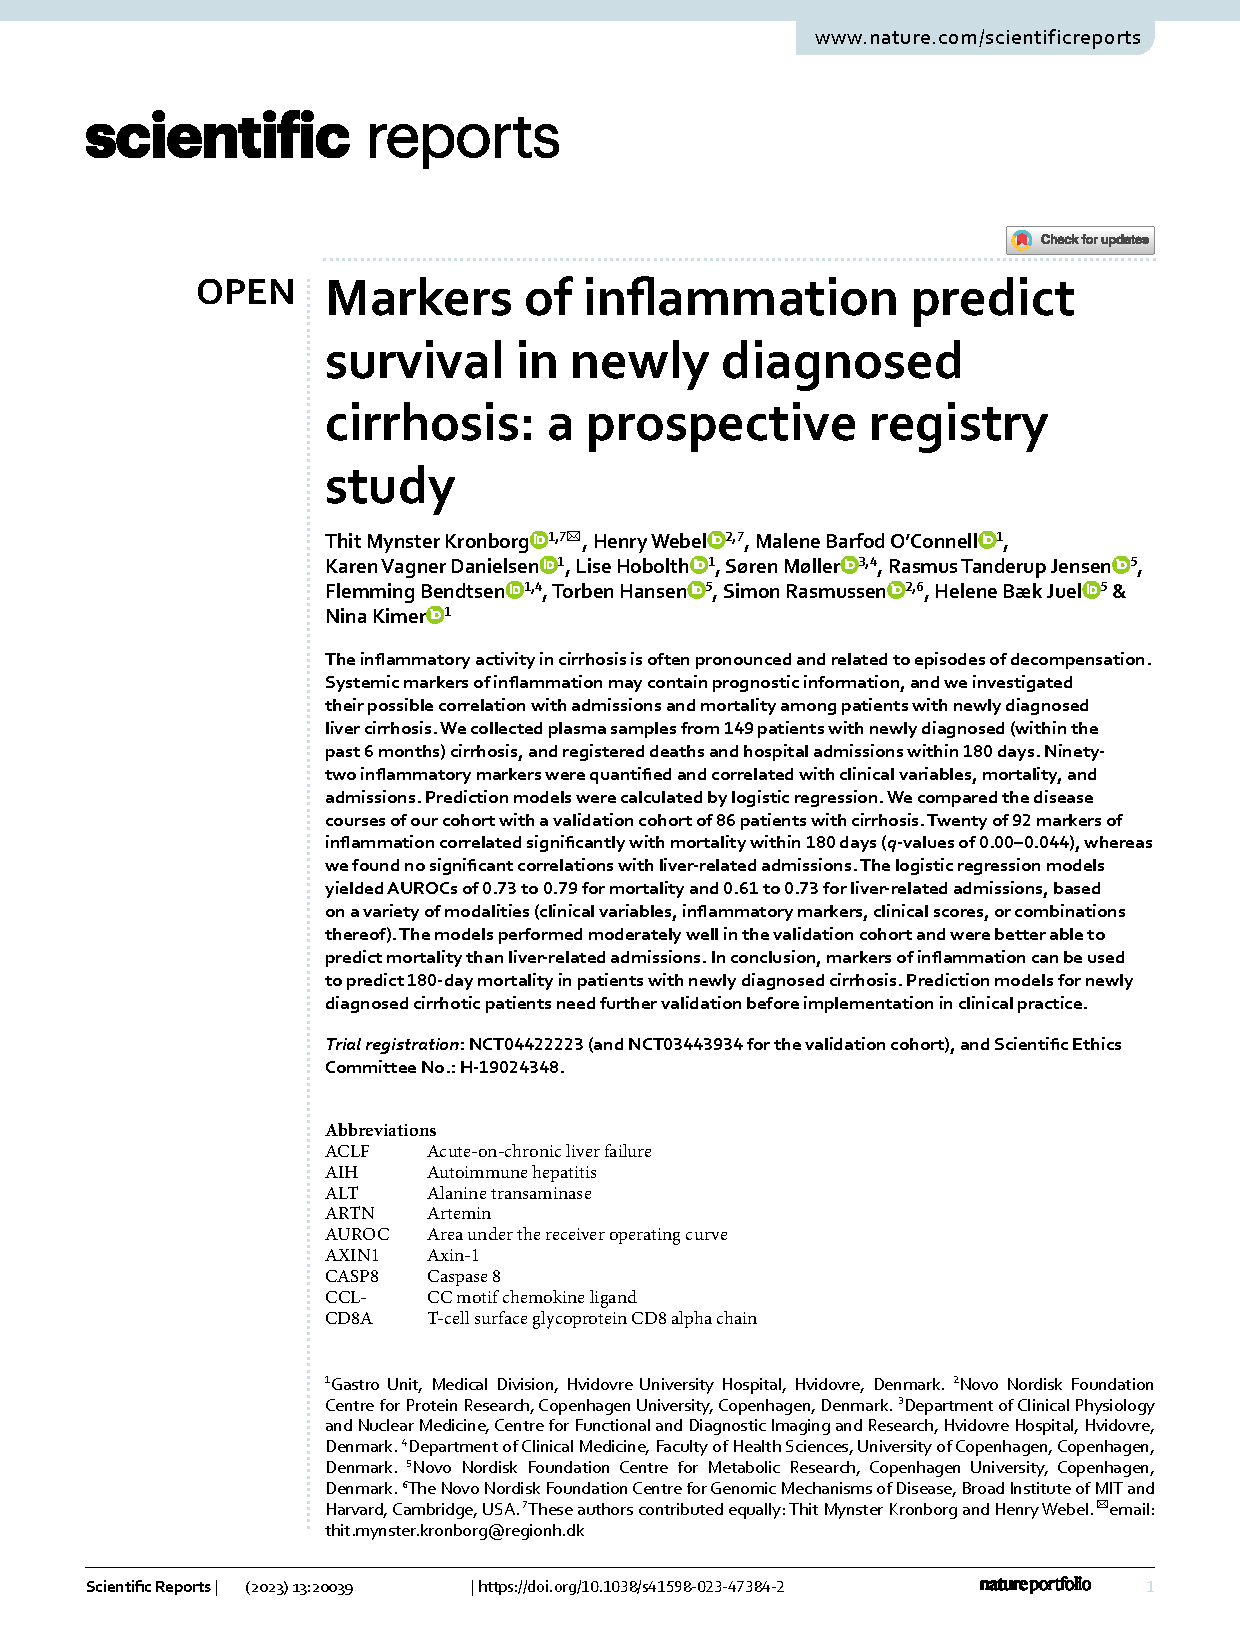
\includepdf[pages=-, ]{papers/s41598-023-47384-2.pdf}
% remove page number:
% 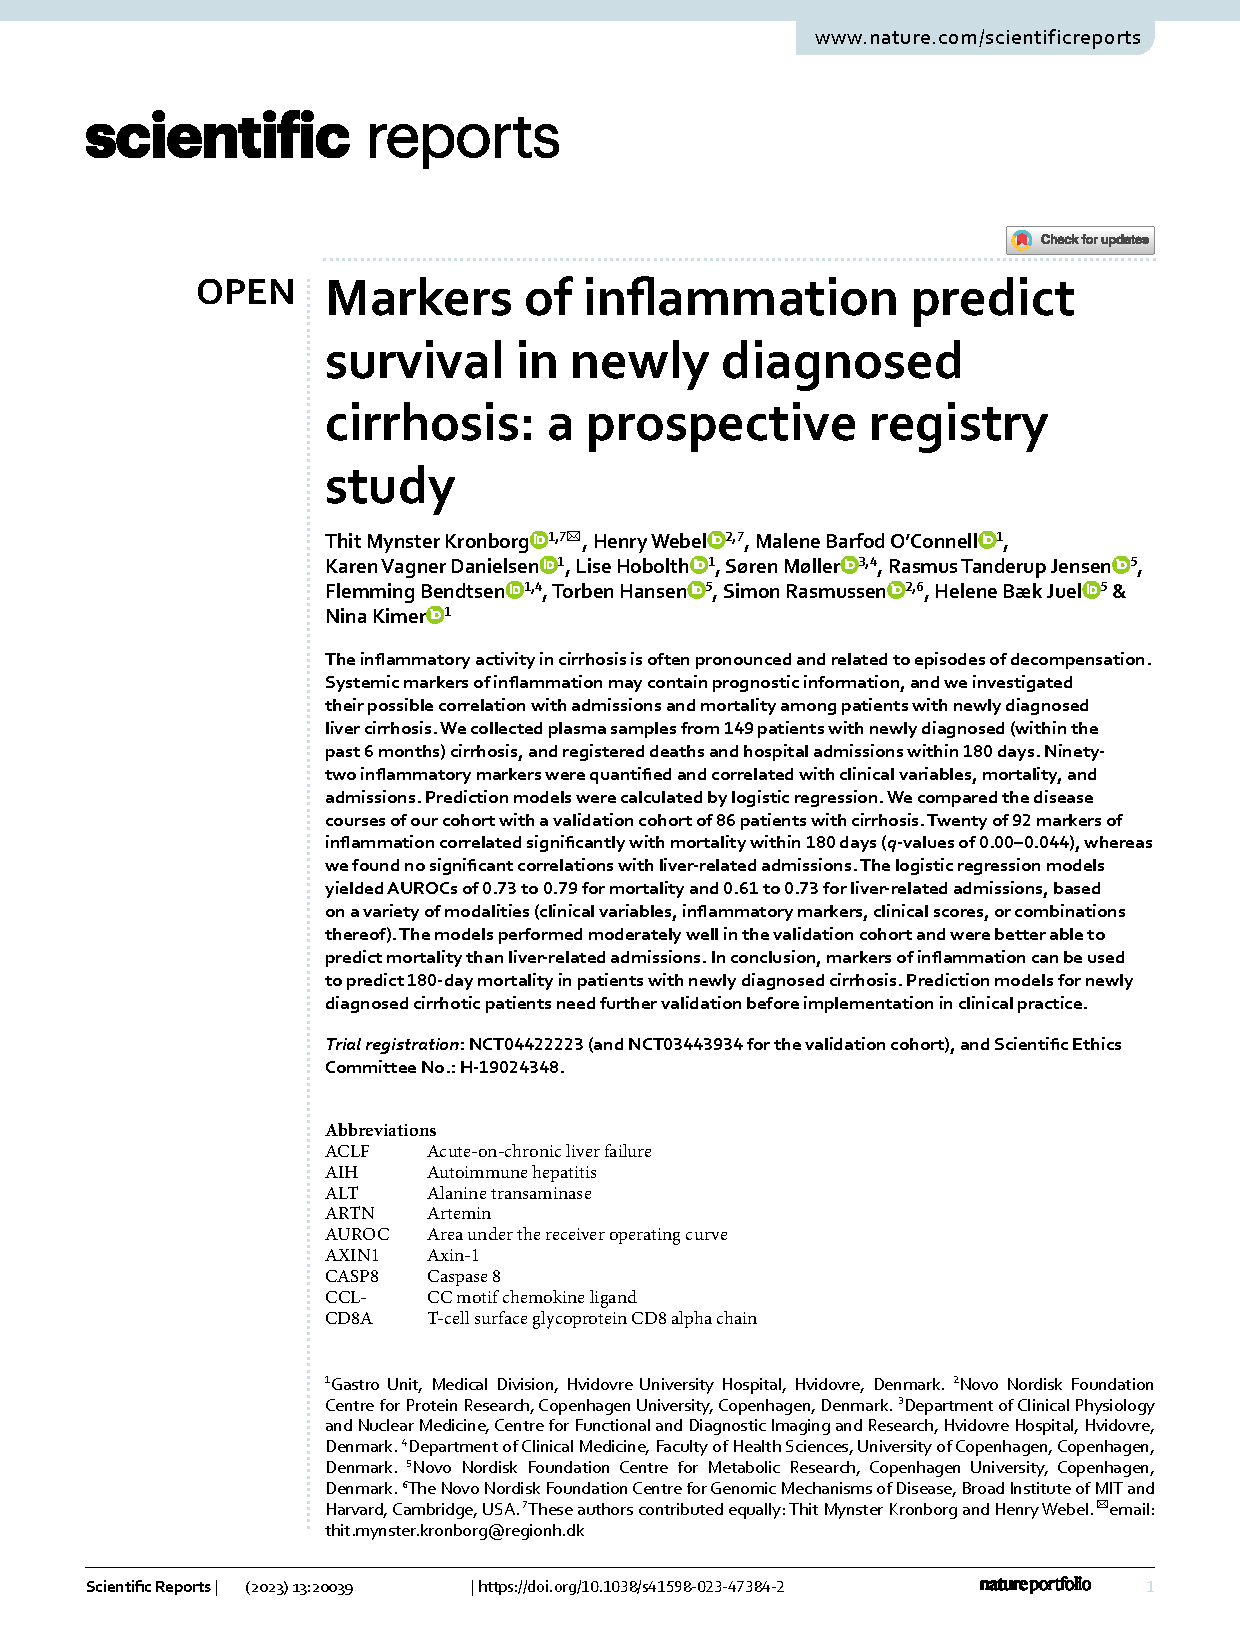
\includepdf[pages=-, pagecommand={\thispagestyle{empty}}]{papers/s41598-023-47384-2.pdf}




%\chapter{Discussion}
\label{chap:disc}
\vspace*{3cm}
\section{Summary of findings}
\Blindtext[1]
\vfill   % INCLUDE Discussion
%\chapter{Conclusion}
\label{chap:con}
\Blindtext[2]
   % INCLUDE Conclusion
% -------------------------- 
% Back matter
% --------------------------
\chapter{References}
\vspace{1cm}
\printbibliography[heading=none]
%\input{frontbackmatter/appendix.tex}


% ********************************************************* 
% END OF THESIS
% *********************************************************
\end{document}